\chapter{Clean Architecture}
Die Clean Architecture ist ein Architekturmuster, das darauf abzielt, Softwareprojekte gut strukturiert, wartbar und testbar zu gestalten. Ein zentrales Thema bei der Entwicklung von Software ist die Wahl zwischen der Verwendung von Libraries und Frameworks. In diesem Kontext wird argumentiert, dass es oft vorteilhafter ist, auf Libraries zurückzugreifen anstatt auf Frameworks zu setzen.\\

\section{Kriterien für nachhaltige Architektur}
\begin{itemize}
\item besitzt einen technologieunabhängigen Kern: der Domain und Applikation ist nur aus Kotlin Code ohne Bibliotheken.
\item behandelt jede Abhängigkeit als temporäre Lösung
\item Unterscheidet zwischen zentralem (\textit{langlebigem}) und peripherem (\textit{kurzlebigem}) Sourcecode
\item \textbf{Metapher:} Die Zwiebel - alle Änderungen sollen den Kern nicht verändern
\end{itemize}

\textbf{Peripherie}: Hier werden die kurzlebigen Bibliotheken an den Kern angebunden. Abhängigkeiten gehen nur vom peripheren Code in den Kern, nie umgekehrt.

\section{Dependency Inversion}
\label{sec:DI}
:Interfaces verwenden damit der Kern Code nicht verändert werden muss. Es kann auch anders gelöst werden die Programmiersprache braucht keine interfaces.
Die Kern-Klasse muss die andere nicht kennen. Schalter(\textbf{Kern}), Schalterbar(\textbf{Plugin}), Lampe/Ventilator(\textbf{Bibliotheken})\\
So in der Theorie.

Um die Dependency Inversion zu erreichen, werden wir eine Abstraktion einführen, die es uns ermöglicht, WordRepository von der konkreten GameLogic-Klasse zu entkoppeln. Wir erstellen eine Schnittstelle für die GameLogic-Klasse und lassen ImplWordRepsoitory stattdessen von dieser Schnittstelle abhängen.

\lstinputlisting[caption={Example for Dependency Inversion}, label={lst:example1}, language=Kotlin]{images/DependencyInversion.kt}

Der Applikation Code ruft Code aus der Adapter Layer auf ohne es zu merken\href{https://github.com/lorenz1702/Spy-Game/commit/280bfad83aeff3a2e16b78514f29b766b8f8259f}{Commit-Hash}. 

Die GameLogic-Klasse kennt also nicht die konkreten Implementierungen der Methoden in den Repositories. Stattdessen verwendet sie die definierten Methoden des Interfaces. Dies ermöglicht eine hohe Flexibilität und Austauschbarkeit der Implementierungen. Zum Beispiel kann die GameLogic-Klasse problemlos mit einer anderen Implementierung des UserRepository arbeiten, solange diese die gleichen Methoden des UserRepository-Interfaces implementiert.
    
Durch die Verwendung von abstrakten Interfaces und die Abhängigkeit von ihnen anstelle von konkreten Implementierungen wird das Prinzip der Dependency Inversion erreicht, was eine lockerere Kopplung und eine bessere Testbarkeit der GameLogic-Klasse ermöglicht.

Hier sieht man noch die Dependency Inversion bildlich dargestellt \ref{fig:14}.

\begin{figure}[h]
    \centering
    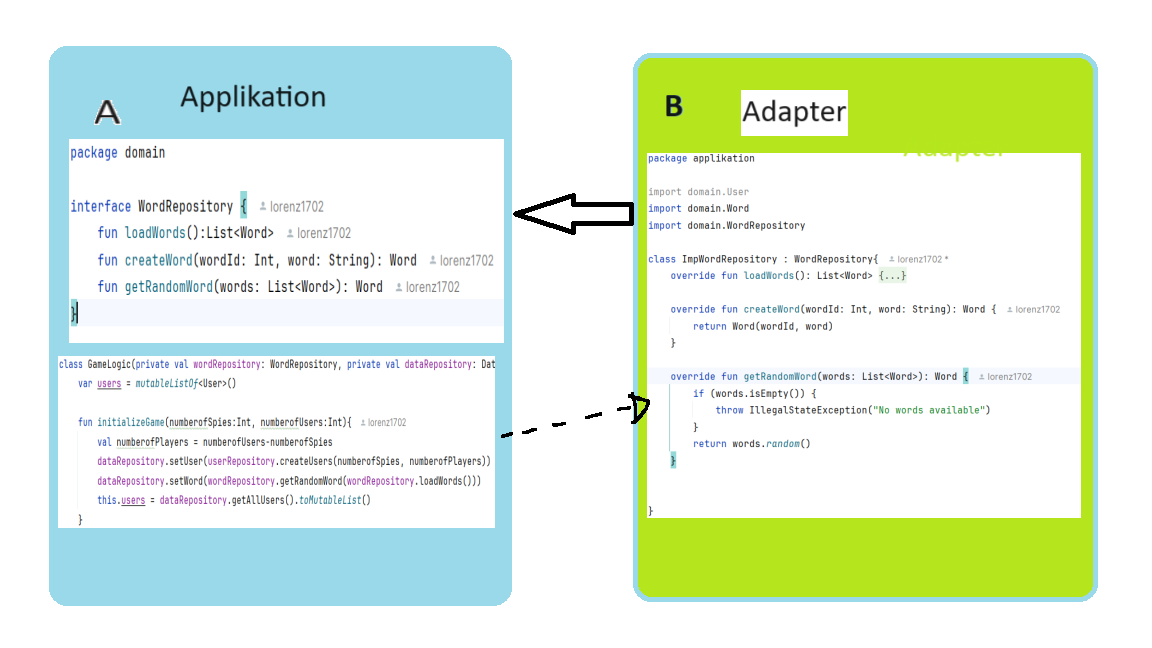
\includegraphics[width=17cm]{images/Denpendancy Inversion.png}
    \caption{Dependency Inversion}%
    \label{fig:14}
\end{figure}

\section{Struktur der Clean Architecture}

\subsection{Domain Code}

In diesem Bereich wird die Benutzer-Entität definiert. 

\subsection{Applikationscode}

Hier werden die Anwendungsfälle (Use Cases) implementiert, die die Kernfunktionalität der Anwendung umsetzen.


\subsection{Plugin}

Adapter dienen als Vermittler zwischen der Daten und der inneren Schicht der Anwendung. Sie übermitteln Daten und führen Aufrufe der inneren Schicht aus. Des Weiteren konvertieren sie Datentypen.



\subsection{Adapter}

Die Adapter-Schicht, die den Ktor-Server implementiert, zeichnet sich durch ihre hohe Austauschbarkeit und Flexibilität aus. Diese Schicht fungiert als Schnittstelle zwischen dem Anwendungskern und dem Ktor-Framework, das für die Verarbeitung von HTTP-Anfragen und -Antworten verantwortlich ist.

Durch die Verwendung des Adaptermusters kann die Implementierung des Ktor-Servers leicht ausgetauscht werden, ohne dass dies Auswirkungen auf den Rest der Anwendung hat. Dies ermöglicht es, verschiedene Implementierungen des Servers zu verwenden, je nach den spezifischen Anforderungen oder Präferenzen des Projekts.

Die Austauschbarkeit der Adapter-Schicht bietet auch die Möglichkeit, verschiedene Technologien oder Frameworks zu evaluieren und zu testen, ohne dass dies größere Änderungen am Anwendungskern erfordert. Dies fördert die Flexibilität und Erweiterbarkeit der Anwendung und erleichtert die Wartung und Weiterentwicklung im Laufe der Zeit.\\

\textbf{Funktionsweise von Serveraufrufen}

Die Funktionalität der Serveraufrufe soll eine Schnittstelle bereitstellen, um Daten zwischen dem Server und der Anwendungslogik auszutauschen.



\subsection{Framework vs. Library}
\textbf{Problem}:
Das Problem von Abhängigkeiten ist, dass sie sich immer ändern, je nach den Frameworks, mit denen man arbeitet. Die verwendeten Frameworks ändern sich alle 5-10 Jahre. Wenn man nicht alle 5 Jahre alles neu machen möchte, muss man die Abhängigkeiten auflösen.

\textbf{Lösung}:
Entscheidungen am besten möglichst spät treffen. \textbf{Minimalziel}:
Entscheidungen müssen revidierbar sein können $\Longrightarrow$ mit möglichst geringen negativen Folgen.

Im Gegensatz dazu bieten Libraries nur spezifische Funktionen oder Werkzeuge, ohne eine vorgegebene Struktur aufzuerlegen. Dies ermöglicht es Entwicklern, die Bibliotheken selektiv und flexibel einzusetzen, je nach den Anforderungen ihres Projekts. Sie bleiben weniger anfällig für Änderungen in der Technologielandschaft, da sie weniger in die Infrastruktur des Projekts eingebettet sind.\\

Durch die Verwendung von Libraries statt Frameworks wird die Abhängigkeit umgekehrt: Statt dass das Projekt von der Funktionsweise des Frameworks abhängt, sind die Libraries von der Implementierung des Projekts abhängig. Dies erhöht die Kontrolle über den Code und erleichtert es, Änderungen vorzunehmen oder Technologien auszutauschen, wenn dies erforderlich ist.\\

In der Clean Architecture wird daher empfohlen, Libraries anstelle von Frameworks zu verwenden, um die Flexibilität, Wartbarkeit und Testbarkeit der Software zu verbessern. Diese Herangehensweise ermöglicht es, die Architektur des Projekts sauber zu halten und die Geschäftslogik von technischen Details zu trennen, was letztendlich zu einer robusteren und skalierbareren Software führt.\\


Um die Dependency Rule der Clean Architecture zu befolgen, habe ich meine Libraries und Frameworks sehr weit nach außen in die äußersten Schichten meines Projekts verschoben. Konkret habe ich die Implementierungsdetails in die Plugin- und Adapter-Schicht ausgelagert. Dadurch wird die innere Geschäftslogik meiner Anwendung von externen Abhängigkeiten isoliert, was die Wartbarkeit und Flexibilität erhöht.\\

Durch die Anwendung der Clean Architecture in meinem Ktor Kotlin Server-Projekt strebe ich danach, einen klaren und gut strukturierten Code zu entwickeln, der leicht zu warten, zu testen und zu erweitern ist. Die klare Trennung der Verantwortlichkeiten und die Verwendung von Libraries anstelle von Frameworks unterstützen dieses Ziel und tragen zu einer langfristig erfolgreichen Entwicklung meines Projekts bei.\\

\href{https://github.com/lorenz1702/Task-Manager/commit/015f5d3147ca527bd73c6bdb2cdf9edba5121b28}{Commit-Hash}


\begin{comment}

\subsection{23.10}
Im Kern kein https, xml, sql er soll nicht wissen das es sie gibt. Dafuer gibt es Adapter.
Warum will man die Werte mundferitg im RenderModel speichern?
\begin{itemize}
    \item Abstraction
    \item Es ist die Letzte Stelle an der ohne Probleme testen können
    \item 
\end{itemize}

Es ist die Letzte Stelle an der ohne Probleme testen können. Wenn ja hat der Kern alles richtig gemacht. Wenn fehler dennoch falsch angezeigt werden wurde es weiter außen falsch gemacht.
Adapter ist falsch kann einfach ersetzt werden. An den Schichtengrenzen kann auf Fehler ueberprueft werden. Die Oberflache mus die Daten nur darstellen.
RenderModel ist wichtig Domainmodel vs Transportmodell. Mit den Plugins kaum beschsaetigen. Und keine erfahrungen mit Frameworks Sammeln.

Mit einer Exception können fehler erkannt werden. Und an die Oberflaeche weiter gegeben werden.

Wie setzt man ein Cleanarchitector Projekt konkrekt um? Der Compiler soll die Pruefung der Abhängigkeit uebernehmen
Jede schicht ist ein eigenes Teil Projekt und sie abstufend von einander abhaengig machen.\\

\textbf{Plugin:} In der Plugin schicht soll so wenig wie möglich selbst schreiben. Möglichst viel von außen nach innen zeigen.
Sie sollen die Daten die geliefert darstellen. Die Plugins sollen nur daten an die Adapter weiter geben.\\

\textbf{Grenzen der Clean Architecture:}
Die Programmiersprache apple ist scheise es ist von der Programmiersprache abhängig und von ARM.

Passwort änderderungs Funktion ist ein USE Case welcher im Applikation Code befindet

User ist eine Entity die befindet sich im Domain Code

\end{comment}